\documentclass[11pt]{article}
\usepackage[margin=1in]{geometry}
\usepackage{amsmath,amssymb}
\usepackage{xcolor}
\usepackage{booktabs}
\usepackage{enumitem}
\usepackage{tikz}
\usetikzlibrary{arrows.meta,positioning,decorations.pathmorphing,calc,shapes.geometric}
\usepackage[colorlinks=true,linkcolor=blue,urlcolor=blue,citecolor=blue]{hyperref}
\usepackage{titlesec}
\titleformat{\section}{\large\bfseries\color{blue!55!black}}{\thesection}{0.6em}{}
\titleformat{\subsection}{\normalsize\bfseries\color{blue!30!black}}{\thesubsection}{0.6em}{}

\newcommand{\quadsum}{\;\oplus\;}
\newcommand{\GeV}{\,\text{GeV}}
\definecolor{boxbg}{rgb}{0.95,0.96,1.0}
\definecolor{warnbg}{rgb}{1.0,0.97,0.90}

% A simple "key idea" box
\newcommand{\keybox}[1]{%
  \begin{center}\fcolorbox{blue!40!black}{boxbg}{%
  \begin{minipage}{0.93\linewidth}\small #1 \end{minipage}}\end{center}}

\title{\vspace{-1.2em}\textbf{The Physics of the Run-24 $p{+}p$ Pion
($\pi^0/\eta$) Nonlinearity Problem}\\[4pt]
\large What ``Resolution'' and ``Smearing'' Mean, and Why PYTHIA Has to be Smeared}
\author{An sPHENIX teaching note (EMCal calibration / PPG12 context)}
\date{2026-06-17}

\begin{document}
\maketitle
\vspace{-1.0em}

\begin{abstract}
\noindent
This note teaches the physics behind a concrete sPHENIX problem: in Run-24
$p{+}p$ collisions at $\sqrt{s}=200\GeV$, the reconstructed $\pi^0$ and $\eta$
mesons in the electromagnetic calorimeter (EMCal) do \emph{not} look the same in
data as in the PYTHIA-8\,+\,GEANT4 simulation. The simulated mass peaks are
\textbf{too narrow} (the MC ``looks too good''), and the energy scale shows a
residual \textbf{nonlinearity} versus transverse momentum. We explain, from
first principles, (i) what \emph{energy resolution} is in a calorimeter, (ii)
what \emph{smearing} of the Monte Carlo (MC) means and why it is needed, (iii)
how the two connect through the standard three-term resolution formula, and (iv)
why a perfectly good simulation must be deliberately ``made worse'' to do honest
physics. All numerical parameters quoted are the ones used in the sPHENIX
EMCal calibration talks and the PPG12 analysis note.
\end{abstract}

\tableofcontents

%================================================================
\section{The measurement and the problem}
%================================================================

sPHENIX reconstructs $\pi^0$ and $\eta$ mesons through their two-photon decay:
\begin{equation}
  \pi^0 \to \gamma\gamma\quad(m_{\pi^0}=0.134977\GeV),\qquad
  \eta  \to \gamma\gamma\quad(m_{\eta}=0.547862\GeV).
\end{equation}
The two photons each deposit their energy as an electromagnetic \emph{shower} in
the EMCal, forming a localized cluster of fired towers. From the two cluster
energies $E_1,E_2$ and their opening angle $\theta_{12}$ we form the
\textbf{two-photon invariant mass}:
\begin{equation}
  M_{\gamma\gamma}=\sqrt{2\,E_1 E_2\,(1-\cos\theta_{12})}.
  \label{eq:mgg}
\end{equation}
Plotting $M_{\gamma\gamma}$ for many photon pairs produces a peak sitting at the
meson mass on top of a combinatorial background. Two numbers are read off the
peak in bins of meson transverse momentum $p_T$:
\begin{itemize}[nosep]
  \item the \textbf{peak position} $M_{\rm fit}$, which tests the EMCal
        \emph{energy scale}. If we plot $M_{\rm fit}/m_{\rm PDG}$ versus $p_T$
        and it is \emph{not flat}, the detector response is
        \textbf{nonlinear} in energy --- this is the ``nonlinearity'' in the
        title.
  \item the \textbf{peak width} $\sigma(M)$, which tests the EMCal
        \emph{energy resolution}. A broad peak means a blurry detector.
\end{itemize}

\keybox{\textbf{The Run-24 $p{+}p$ symptom.} When data are overlaid on the
nominal PYTHIA$+$GEANT4 simulation, \emph{the data peak is much wider than the
simulated peak}, and $M_{\rm fit}/m_{\rm PDG}$ drifts with $p_T$ by a couple of
percent. The simulation is therefore both too sharp (resolution problem) and
slightly mis-scaled (nonlinearity problem). The fix has two independent knobs:
\textbf{smearing} to widen the MC peak, and an \textbf{energy-scale /
nonlinearity correction} to re-center it.}

Why does this matter? Because the final physics result --- e.g.\ the PPG12
isolated-prompt-photon cross section, or a $\pi^0/\eta$ spectrum --- is obtained
by \emph{comparing data to a simulation}. Efficiencies, backgrounds, and the
\emph{unfolding} that corrects detector smearing back to truth are all computed
from the MC. If the MC does not reproduce the true detector resolution and
scale, every one of those corrections is biased. The simulation must tell the
truth about how good (and how bad) the real detector is.

%================================================================
\section{Energy resolution: what ``blurry'' means quantitatively}
%================================================================

\subsection{The definition}
Send a photon of a \emph{fixed} true energy $E$ into the calorimeter many times.
The reconstructed energies do not all come back equal; they scatter in a roughly
Gaussian cloud of width $\sigma_E$ around a mean. The \textbf{energy resolution}
is the fractional width
\begin{equation}
  \frac{\sigma_E}{E}.
\end{equation}
A small $\sigma_E/E$ means a sharp, well-measured detector; a large value means a
blurry one. Crucially, the resolution is \emph{not} a single number --- it
depends on energy, and that dependence carries physics.

\subsection{The three-term calorimeter formula}
For a sampling calorimeter like the sPHENIX EMCal (a tungsten--scintillating-fiber
``SPACAL''), the resolution is parameterized by three terms added \emph{in
quadrature}:
\begin{equation}
  \boxed{\;\frac{\sigma_E}{E}
   = \sqrt{\;\frac{p_0^2}{E}\;+\;\frac{p_1^2}{E^2}\;+\;p_2^2\;}
   \;\equiv\; \frac{p_0}{\sqrt{E}}\quadsum\frac{p_1}{E}\quadsum p_2\;}
  \qquad (E\ \text{in GeV}),
  \label{eq:reso}
\end{equation}
where ``$\oplus$'' denotes addition in quadrature. Each term is a distinct piece
of physics:
\begin{description}[leftmargin=2.2em]
  \item[\;$p_0/\sqrt{E}$ --- stochastic (sampling) term.] Comes from
        \emph{statistical fluctuations} in the shower: how many shower particles
        cross active scintillator, how many scintillation photons are made, how
        many photoelectrons the SiPMs detect. These are Poisson-like, so the
        relative fluctuation scales as $1/\sqrt{N}\propto 1/\sqrt{E}$. It
        \textbf{shrinks} as energy rises --- high-energy showers are measured
        \emph{proportionally} better.
  \item[\;$p_1/E$ --- noise term.] Electronic noise and pileup add a roughly
        \emph{fixed} amount of energy regardless of the signal, so as a
        \emph{fraction} it falls like $1/E$. It matters only at low energy and is
        often negligible (here $p_1$ is small or zero).
  \item[\;$p_2$ --- constant term.] Comes from effects that scale \emph{with}
        the energy: calibration spread tower-to-tower, light-collection
        non-uniformity, shower leakage out the back/sides, and dead material.
        Being a fixed fraction, it does \textbf{not} shrink with energy and
        therefore \textbf{dominates the resolution at high $E$}.
\end{description}

\begin{center}
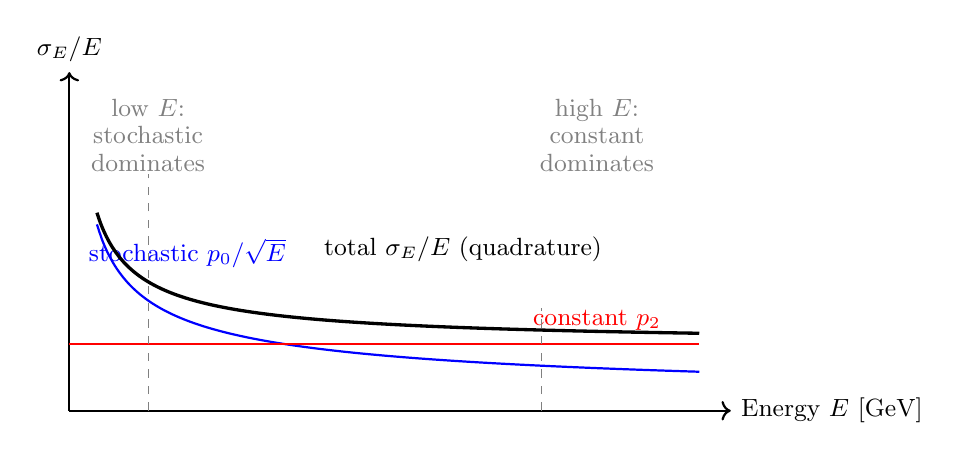
\begin{tikzpicture}[scale=1.0]
  % axes
  \draw[->,thick] (0,0) -- (8.4,0) node[right] {\small Energy $E$ [GeV]};
  \draw[->,thick] (0,0) -- (0,4.3) node[above] {\small $\sigma_E/E$};
  % stochastic term  ~ p0/sqrt(E)
  \draw[blue,thick,domain=0.35:8,samples=120,smooth] plot (\x,{1.4/sqrt(\x)});
  \node[blue] at (1.5,2.0) {\small stochastic $p_0/\sqrt{E}$};
  % constant term  p2
  \draw[red,thick] (0,0.85) -- (8,0.85);
  \node[red] at (6.7,1.15) {\small constant $p_2$};
  % total (quadrature)
  \draw[black,very thick,domain=0.35:8,samples=160,smooth]
        plot (\x,{sqrt( (1.4/sqrt(\x))^2 + 0.85^2 )});
  \node[black] at (5.0,2.05) {\small total $\sigma_E/E$ (quadrature)};
  % annotate regimes
  \draw[dashed,gray] (1.0,0) -- (1.0,3.0);
  \node[gray,align=center] at (1.0,3.5) {\small low $E$:\\[-2pt]\small stochastic\\[-2pt]\small dominates};
  \draw[dashed,gray] (6.0,0) -- (6.0,1.3);
  \node[gray,align=center] at (6.7,3.5) {\small high $E$:\\[-2pt]\small constant\\[-2pt]\small dominates};
\end{tikzpicture}
\end{center}
\noindent\textit{Figure 1. Schematic of the three-term resolution. The
stochastic term (blue) falls as $1/\sqrt{E}$; the constant term (red) is flat;
their quadrature sum (black) is the measured resolution. At high energy the
constant term sets the floor --- which is exactly where the Run-24 data/MC
disagreement lives.}

\subsection{From photon resolution to meson width}
Because Eq.~\eqref{eq:mgg} multiplies the two photon energies, the
\emph{meson} relative width inherits the photon resolution. For symmetric
decays one finds, to good approximation,
\begin{equation}
  \frac{\sigma(M)}{M}\;\approx\;\frac{1}{\sqrt{2}}\,\frac{\sigma_E}{E}\;
  \oplus\;(\text{angular / position term}),
\end{equation}
so the \emph{width of the $\pi^0/\eta$ peak versus $p_T$} is a direct,
data-accessible measurement of the EMCal energy (and position) resolution. This
is the experimental handle the calibration team uses: fit the peak in each $p_T$
slice, plot $\sigma(M)/M$ vs $p_T$, and read off the resolution. The reference
sPHENIX single-photon (test-beam) resolution is
\begin{equation}
  \frac{\sigma_E}{E}\;\approx\;\frac{16\%}{\sqrt{E}}\quadsum 5\%,
\end{equation}
i.e.\ $p_0\approx0.16$, $p_2\approx0.05$.

%================================================================
\section{Why PYTHIA needs ``smearing''}
%================================================================

\subsection{What PYTHIA and the MC chain actually do}
PYTHIA-8 (Detroit tune) generates the $p{+}p$ collision: it produces the
partons, hadronizes them, and outputs a list of final-state particles with
\emph{exact, truth-level} four-momenta. PYTHIA itself knows nothing about the
detector --- it is pure event generation. Those truth particles are then passed
to \textbf{GEANT4}, which simulates the showers in the EMCal, and finally the
same reconstruction used on data turns the simulated energy deposits into
clusters and meson candidates.

\keybox{\textbf{The core issue.} ``PYTHIA smearing'' is shorthand for the whole
PYTHIA$+$GEANT4$+$reco simulation chain, and the empirical fact that
\emph{its reconstructed energy resolution is better (narrower) than the real
detector's}. The simulated EMCal is intrinsically too clean: fitting the
unsmeared MC photon response gives a resolution like
$\sigma_E/E\approx 0.185/\sqrt{E}\oplus 0.040$ --- note the very small constant
term $p_2\approx0.04$. Real Run-24 data want a constant term closer to
$0.05$--$0.08$. The MC peak is therefore sharper than data, and no honest
comparison is possible until the MC is broadened to match.}

Why is the simulation too good? In practice, real detectors carry imperfections
that are hard to capture fully in GEANT4: tower-to-tower miscalibration spread,
light-collection non-uniformity along the fibers, SiPM-to-SiPM gain variation,
subtle dead/edge material, and time-dependent effects in a real run. These
inflate the \emph{constant term} $p_2$ in data above what the idealized
simulation produces. (The calibration talks note candidly that it is ``unclear''
exactly which effect dominates --- which is precisely why the correction is
applied empirically.)

\subsection{What ``smearing'' is}
\textbf{Smearing} is the deliberate, controlled \emph{degradation} of a
simulated quantity so that the MC reproduces the worse resolution of real data.
It is the mirror image of resolution: resolution \emph{measures} the blur;
smearing \emph{injects} the blur into an otherwise-too-perfect simulation.

Operationally, each simulated photon (or cluster) energy is multiplied by a
random Gaussian factor centered on one:
\begin{equation}
  E \;\longrightarrow\; E\cdot f,\qquad
  f\sim \mathrm{Gaus}\!\big(1,\ \sigma_{\rm extra}(E)\big).
  \label{eq:smear}
\end{equation}
The width $\sigma_{\rm extra}$ is \emph{not} the full data resolution --- the MC
already has its own intrinsic resolution. We only need to add the
\emph{missing} amount, computed as the \textbf{quadrature difference} between the
target (data) resolution and what the MC already has:
\begin{equation}
  \boxed{\;\sigma_{\rm extra}(E)=\sqrt{\,\max\!\big(0,\;
  \sigma_{\rm data}^2(E)-\sigma_{\rm MC}^2(E)\big)}\;}
  \label{eq:quaddiff}
\end{equation}
The $\max(0,\cdot)$ guards against the (unphysical) case where the MC is already
wider than data --- you can broaden a distribution but you cannot sharpen it by
adding random noise. The position (angle) of the photon is smeared the same way,
but \emph{additively} on $\eta$ and $\phi$ and centered at zero:
$\eta\to\eta+\mathrm{Gaus}(0,\sigma_\psi)$, similarly for $\phi$.

\begin{center}
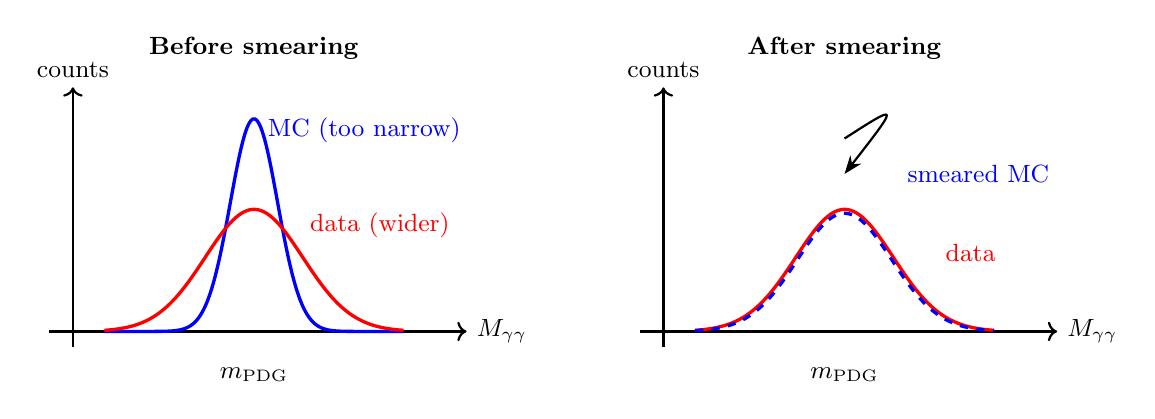
\begin{tikzpicture}[scale=1.0]
  \begin{scope}
    % MC narrow peak
    \draw[->,thick] (-0.3,0) -- (5.0,0) node[right]{\small $M_{\gamma\gamma}$};
    \draw[->,thick] (0,-0.2) -- (0,3.1) node[above]{\small counts};
    % narrow gaussian (MC), centered 2.3
    \draw[blue,very thick,domain=0.4:4.2,samples=160,smooth]
       plot (\x,{2.7*exp(-(\x-2.3)^2/(2*0.30^2))});
    % wide gaussian (data), centered 2.3
    \draw[red,very thick,domain=0.4:4.2,samples=160,smooth]
       plot (\x,{1.55*exp(-(\x-2.3)^2/(2*0.62^2))});
    \node[blue] at (3.7,2.55) {\small MC (too narrow)};
    \node[red]  at (3.9,1.35) {\small data (wider)};
    \node at (2.3,-0.55) {\small $m_{\rm PDG}$};
    \node[align=center] at (2.3,3.6) {\small \textbf{Before smearing}};
  \end{scope}
  \begin{scope}[xshift=7.5cm]
    \draw[->,thick] (-0.3,0) -- (5.0,0) node[right]{\small $M_{\gamma\gamma}$};
    \draw[->,thick] (0,-0.2) -- (0,3.1) node[above]{\small counts};
    % both wide now, overlapping
    \draw[red,very thick,domain=0.4:4.2,samples=160,smooth]
       plot (\x,{1.55*exp(-(\x-2.3)^2/(2*0.62^2))});
    \draw[blue,very thick,dashed,domain=0.4:4.2,samples=160,smooth]
       plot (\x,{1.50*exp(-(\x-2.3)^2/(2*0.60^2))});
    \node[blue] at (4.0,2.0) {\small smeared MC};
    \node[red]  at (3.9,1.0) {\small data};
    \node at (2.3,-0.55) {\small $m_{\rm PDG}$};
    \node[align=center] at (2.3,3.6) {\small \textbf{After smearing}};
    % arrow indicating broadening
    \draw[->,thick,>=Stealth] (2.3,2.45) .. controls (3.0,2.9) .. (2.3,2.0);
  \end{scope}
\end{tikzpicture}
\end{center}
\noindent\textit{Figure 2. The role of smearing. Left: the nominal MC peak
(blue) is sharper than the data peak (red) --- this is the symptom. Right: after
injecting $\sigma_{\rm extra}$ via Eq.~\eqref{eq:smear}, the MC width (blue
dashed) is broadened to match data. Smearing changes the \emph{width}, not the
\emph{center}; re-centering is the separate energy-scale job.}

\subsection{The smearing parameters actually used}
The data target and MC resolutions are each fit to the three-term form
Eq.~\eqref{eq:reso}. The numbers used in the sPHENIX calibration talks and the
PPG12 analysis note are:

\begin{center}
\renewcommand{\arraystretch}{1.25}
\begin{tabular}{l c c c}
\toprule
\textbf{Resolution set} & $\boldsymbol{p_0}$ ($/\sqrt{E}$) & $\boldsymbol{p_1}$ ($/E$) & $\boldsymbol{p_2}$ (const)\\
\midrule
PYTHIA intrinsic / MC  (too narrow)        & 0.185 & 0.00  & 0.040 \\
\textbf{nominal} data target               & 0.15  & 0.05  & 0.05  \\
``wider-data'' variation (systematic)      & 0.13  & 0.08  & 0.08  \\
tuned working set (``smear11'')            & 0.180 & 0.020 & 0.015 \\
test-beam single-$\gamma$ reference        & 0.16  & --    & 0.05  \\
\bottomrule
\end{tabular}
\end{center}

\noindent Reading the physics out of the table:
\begin{itemize}[nosep]
  \item The MC's constant term ($p_2\!=\!0.04$) is smaller than data's
        ($p_2\!=\!0.05$--$0.08$). That gap \emph{at high energy} is the entire
        problem, because the constant term is the high-$E$ floor (Fig.~1).
  \item With the nominal target, $\sigma_{\rm extra}$ from
        Eq.~\eqref{eq:quaddiff} is $\approx 0$ below $\sim$17\GeV{} and rises to
        only $\sim$2\% above 20\GeV. \textbf{Smearing barely matters at low
        $p_T$ and matters most at high $p_T$} --- consistent with the
        constant-term picture.
  \item The ``wider-data'' variation gives $\sigma_{\rm extra}\!\approx\!6\%$
        roughly flat in energy. The spread between ``no extra smearing'' and
        ``wider-data'' is taken as the \emph{energy-resolution systematic} (the
        PPG12 ``eres'' uncertainty), reaching $\pm9.6\%$ near $E_T\!\sim\!27\GeV$.
\end{itemize}

The position smearing pairs with the above:
\begin{equation}
  \sigma_\psi(E)=0.0030/\sqrt{E}\quadsum 0.0040\ \ (\text{tuned}),\qquad
  \sigma_\psi(E)=0.0055/\sqrt{E}\quadsum 0.0020\ \ (\text{data-driven}),
\end{equation}
and a small energy-scale factor $E_{\rm scale}=f(E)\times0.998$ re-centers the
peak (the nonlinearity knob, Sec.~\ref{sec:nonlin}).

\subsection{The ``smearN'' samples}
The simulation samples are named by their smearing recipe. The MC is fit, the
quadrature-difference smear functions are stored, and applied photon-by-photon:
\begin{itemize}[nosep]
  \item \texttt{pythia\_smear1} --- ``global minimum difference'' set.
  \item \texttt{pythia\_smear2} --- extra constant $c_E=0.08$; found
        \emph{insufficient} (MC still too narrow).
  \item \texttt{pythia\_smear3} --- extra constant $c_E=0.05$.
  \item \texttt{pythia\_smear5} --- ``added an additional 8\% energy smearing'';
        the nominal sample; width agreement at the MC statistical limit.
  \item \texttt{pythia\_smear11} --- ``added an additional $8\%/\sqrt{E}$''
        (i.e.\ an extra \emph{stochastic} term, not a flat constant); the newest,
        leaving only a $\sim$2\% high-$p_T$ $\eta$ residual.
  \item \texttt{pythia\_smear5\_pix} --- \texttt{smear5} plus the SiPM
        pixel-occupancy nonlinearity (Sec.~\ref{sec:nonlin}).
\end{itemize}
The recurring ``$\sim$8\% smearing'' is just the extra $\sim$0.08 resolution
term needed to widen the intrinsically narrow PYTHIA peak up to the data width.

%================================================================
\section{The nonlinearity: re-centering the peak}
\label{sec:nonlin}
%================================================================

Smearing fixes the \emph{width}; a separate correction fixes the \emph{mean}.
A calorimeter is \textbf{nonlinear} if the reconstructed energy is not a constant
fraction of the true energy --- i.e.\ if $M_{\rm fit}/m_{\rm PDG}$ drifts with
$p_T$. Two real, physical effects drive a mild nonlinearity in the sPHENIX EMCal,
and both are added to the MC so it can describe data:

\begin{description}[leftmargin=1.6em]
  \item[(1) Longitudinal light attenuation in the SPACAL fibers.]
    A higher-energy shower develops \emph{deeper} in the calorimeter (its
    maximum sits at depth $t_{\max}\sim X_0\ln E$). Light produced deeper has a
    longer path to the SiPMs at the back, so more of it is attenuated:
    \begin{equation}
      \frac{S(E)}{E}\;\sim\;e^{-\Delta x/\Lambda}\;\sim\;E^{-X_0/\Lambda},
      \qquad \Lambda\approx1.6\ \text{m (TDR)}.
    \end{equation}
    This costs roughly $1.0\%/1.3\%/1.6\%$ of response at $10/20/40\GeV$ ---
    a slow droop of the energy scale with energy. It is implemented as a
    $z$-dependent light efficiency in the MC.

  \item[(2) SiPM pixel saturation / occupancy.]
    Each tower's SiPMs have a finite number of pixels,
    $N_{\rm pix}\!\sim\!1.6\times10^5$ (4 SiPMs $\times\sim$40k each), and fire
    $\sim$400--500 photoelectrons per GeV. As energy rises, an increasing
    fraction of pixels are already lit, so the response saturates. A first-order
    estimate gives $\sim$0.125\%$\times E$, i.e.\ $\sim$1.25/2.5/5\% at
    $10/20/40\GeV$. This was missing from the nominal MC and is now added
    (validated against test-beam data) via \texttt{pythia\_smear5\_pix}.
\end{description}

\begin{center}
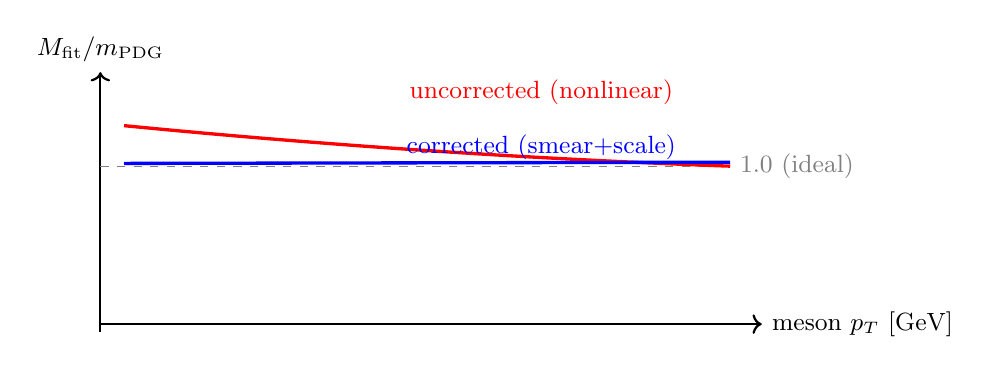
\begin{tikzpicture}[scale=1.0]
  \draw[->,thick] (0,0) -- (8.4,0) node[right]{\small meson $p_T$ [GeV]};
  \draw[->,thick] (0,-0.1) -- (0,3.2) node[above]{\small $M_{\rm fit}/m_{\rm PDG}$};
  % ideal line at 1.0
  \draw[dashed,gray] (0,2.0) -- (8,2.0) node[right,gray]{\small $1.0$ (ideal)};
  % nonlinear droop (uncorrected) - starts ~1.04, droops
  \draw[red,very thick,domain=0.3:8,samples=120,smooth]
        plot (\x,{2.0 + 0.55 - 0.10*\x + 0.004*\x*\x});
  \node[red] at (5.6,2.95) {\small uncorrected (nonlinear)};
  % corrected - flat near 1.01
  \draw[blue,very thick,domain=0.3:8,samples=80,smooth]
        plot (\x,{2.0 + 0.04 + 0.002*\x});
  \node[blue] at (5.6,2.25) {\small corrected (smear+scale)};
\end{tikzpicture}
\end{center}
\noindent\textit{Figure 3. Schematic of the nonlinearity. Without the
attenuation and pixel-saturation corrections, the reconstructed mass scale
$M_{\rm fit}/m_{\rm PDG}$ drifts with $p_T$ (red). With the MC scale correction
$E_{\rm scale}=f(E)\times0.998$ and the added physical effects, it is flat and
close to unity (blue). This is a schematic, not measured data.}

After tuning, the residual high-$p_T$ $\eta$ discrepancy is only about
$2$--$2.5\%$, which is what the calibration update flags as the remaining
``nonlinearity'' to investigate.

%================================================================
\section{Why this matters downstream: smearing feeds unfolding}
%================================================================

A measured spectrum is the true spectrum \emph{convolved} with detector effects
(resolution, smearing, bin migration, efficiency). \textbf{Unfolding} is the
statistical inversion that recovers truth from the measured distribution. With a
\emph{response matrix} $R_{ij}=P(\text{measured }i\,|\,\text{truth }j)$ built
from MC,
\begin{equation}
  \vec m = R\,\vec t \quad\Longrightarrow\quad
  \vec t_{\rm unfold}=\mathcal{U}(R,\vec m),
\end{equation}
solved with iterative Bayesian (D'Agostini) unfolding to avoid noise
amplification. The response matrix $R$ \emph{is built from the MC}. If the MC
resolution is wrong --- too narrow --- then $R$ underestimates the true bin
migration, and the unfolded result is biased. Toy studies in the sPHENIX work
area deliberately mismatch the MC and data resolutions and show the unfolding
bias grow as the mismatch grows. \textbf{This is the quantitative reason
smearing must be tuned first}: an honest cross section (e.g.\ PPG12 isolated
photons) requires a response matrix built from a simulation that has the same
resolution as the data.

\keybox{\textbf{One-line glossary.}\\
\emph{Resolution} = how blurry the detector is (measured from the $\pi^0/\eta$
peak width).\\
\emph{Smearing} = injecting exactly the missing blur into the too-clean MC, via
$E\to E\cdot\mathrm{Gaus}(1,\sigma_{\rm extra})$ with
$\sigma_{\rm extra}=\sqrt{\sigma_{\rm data}^2-\sigma_{\rm MC}^2}$.\\
\emph{Nonlinearity} = the energy scale drifting with $p_T$, fixed by a separate
$E_{\rm scale}$ correction plus added physical effects (fiber attenuation, SiPM
saturation).\\
\emph{Unfolding} = removing the detector blur from a measured spectrum to recover
truth --- which only works if the MC used to build it was smeared to match data.}

%================================================================
\section{Summary}
%================================================================
\begin{enumerate}[nosep]
  \item In Run-24 $p{+}p$, the reconstructed $\pi^0/\eta$ peaks are
        \emph{wider in data than in PYTHIA$+$GEANT4} (resolution mismatch) and
        the mass scale drifts slightly with $p_T$ (nonlinearity).
  \item Resolution follows
        $\sigma_E/E=p_0/\sqrt{E}\oplus p_1/E\oplus p_2$; the data/MC gap lives in
        the \emph{constant term} $p_2$, so it grows at high $p_T$.
  \item ``PYTHIA smearing'' means broadening the too-clean simulated energy by a
        Gaussian factor of width
        $\sigma_{\rm extra}=\sqrt{\sigma_{\rm data}^2-\sigma_{\rm MC}^2}$, with
        the working set $\sigma_E/E\approx0.18/\sqrt{E}\oplus0.02/E\oplus0.015$
        (sample ``smear11'', the recurring ``$\sim$8\%'' extra term).
  \item The nonlinearity is re-centered with $E_{\rm scale}=f(E)\times0.998$ plus
        two physical effects in the MC: longitudinal fiber light attenuation and
        SiPM pixel saturation.
  \item All of this is required because the MC builds the efficiency,
        background, and \emph{unfolding} corrections for the final cross section;
        a simulation that does not reproduce the real resolution would bias the
        physics result.
\end{enumerate}

\bigskip
\noindent\footnotesize Numerical parameters are taken from the sPHENIX EMCal
calibration update talks (B.~Seidlitz) and the PPG12 analysis note
(sPH-ppg-2024-012, v4). Figures here are hand-drawn TikZ schematics intended to
illustrate the concepts; they are not measured data plots.

\end{document}
